\documentclass[11pt,twoside,a4paper]{article}
\usepackage{amsmath,amsfonts}
\usepackage{algorithmic}
\usepackage{algorithm}
\usepackage{array}
\usepackage[caption=false,font=normalsize,labelfont=sf,textfont=sf]{subfig}
\usepackage{textcomp}
\usepackage{stfloats}
\usepackage{ctex}
\usepackage{url}
\usepackage{verbatim}
\usepackage{graphicx}
\usepackage{cite}
\usepackage{amsmath,amsfonts}
\usepackage{algorithmic}
\usepackage{algorithm}
\usepackage{array}
\usepackage[caption=false,font=normalsize,labelfont=sf,textfont=sf]{subfig}
\usepackage{textcomp}
\usepackage{stfloats}
\usepackage{url}
\usepackage{verbatim}
\usepackage{graphicx}
\usepackage{cite}
\usepackage{mathptmx}
\usepackage[justification=centering]{caption}
\usepackage[T1]{fontenc}
\usepackage{hyperref}
\usepackage{amssymb}
\usepackage{float}
\usepackage{subcaption}
\begin{document}
	\section{模型假设和约定}
	
	\section{符号说明}
	
	\section{基本模型建立}
\subsection{多波束测线二维平面模型}
	\begin{figure}[htbp]
		\centering
		\includegraphics[scale=1.5]{3}
		\caption{多波束探测的工作原理}
		\label{1}
	\end{figure}
	
	多波束探测系统在与航迹垂直的平面内发射多个波束,其工作原理如图\ref{1}所示,在海底平坦的海域,其能够测出以测线为轴线具有一定宽度的全覆盖水深条带,其覆盖宽度$W$随换能器开角$\theta$和水深$D$的变化而变化
	\begin{equation}
		W=2 \times D \tan{\frac{\theta}{2}} \text{。}
	\end{equation}	
	\begin{figure}[h]
		\centering
		\includegraphics[scale=0.4]{6}
		\caption{覆盖宽度、测线间距和重叠率之间的关系}
		\label{3}	
	\end{figure}

若两个测线相互平行,如图 \ref{3}所示,其重叠率$\eta$可表示为对于每个覆盖宽度$W$的重叠宽度$W_\text{ 重}$与覆盖宽度总和的比值,即
	\begin{equation}
	\eta=\frac{W_\text{重} \times 2}{W+W}
	\label{eq2}
    \end{equation}
其中 $W_\text{重}=2\times\frac{W}{2}-d$,
经化简得
	\begin{equation}
	\eta=1-\frac{d}{W}
   \end{equation}



\begin{figure}[h]
	\centering
	\includegraphics[scale=0.9]{4}
	\caption{单测线斜坡中多波束探测的工作原理1}
	\label{2}
\end{figure}

 \begin{figure}[h]
	\centering
	\includegraphics[scale=0.9]{7}
	\caption{单测线斜坡中多波束探测的工作原理2}
	\label{5}
\end{figure}



	 对于坡度为$\alpha$的海底坡面,如图\ref{2}和图\ref{5} 所示,其覆盖宽度 $W$由侧线为轴线的左侧宽度$W_1$ 和右侧宽度$W_2$组成。对于左侧宽度$W_1$有
	
	 \begin{equation}
		\frac{D}{\sin \left(\frac{1}{2}\times \pi -\alpha-\frac{1}{2}\times \theta \right)}=\frac{W_1}{\sin( \frac{1}{2}\times \theta)} \text{。}
	 \end{equation}
	 经化简得
	 	 \begin{equation}
	  W_1=\frac{D \sin{(\frac{\theta}{2}})}{\cos{(\frac{\theta}{2}+\alpha})}
	 	\end{equation}
 	同理,对于右侧宽度$W_2$
 	 \begin{equation}
 		\frac{D}{\sin \left(\frac{1}{2}\times \pi +\alpha-\frac{1}{2}\times \theta \right)}=\frac{W_2}{\sin( \frac{1}{2}\times \theta)} \text{。}
 	\end{equation}
     经化简得
      \begin{equation}
     	W_2=\frac{D \sin{(\frac{\theta}{2}})}{\cos{(\alpha-\frac{\theta}{2}})}
     \end{equation}
    由此可得
     \begin{equation}
    	W=\frac{D \sin{(\frac{\theta}{2}})}{\cos{(\alpha-\frac{\theta}{2}})}+\frac{D \sin{(\frac{\theta}{2}})}{\cos{(\alpha+\frac{\theta}{2}})}
    	\label{eq1}
    \end{equation}
 
	
		\begin{figure}[h]
		\centering
		\includegraphics[scale=1]{5}
		\caption{双测线斜坡中多波束探测的工作原理}
		\label{4}
	\end{figure}
对于双测线工作的情况, 如图\ref{4}所示,根据公式(\ref{eq1}),
 \begin{equation}
	W_\text{测1}=\frac{D_1 \sin{(\frac{\theta}{2}})}{\cos{(\alpha-\frac{\theta}{2}})}+\frac{D_1 \sin{(\frac{\theta}{2}})}{\cos{(\alpha+\frac{\theta}{2}})}
\end{equation}	
 \begin{equation}
	W_\text{测2}=\frac{D_2 \sin{(\frac{\theta}{2}})}{\cos{(\alpha-\frac{\theta}{2}})}+\frac{D_2 \sin{(\frac{\theta}{2}})}{\cos{(\alpha+\frac{\theta}{2}})}
\end{equation}	
	$W_\text{测1}$ 和	$W_\text{测2}$ 之间的重叠面积$W_\text{重}$可以表示为
 \begin{equation}
 W_\text{重}=(1-\frac{\beta-d}{\beta})\frac{D}{sin{\alpha}}
\end{equation}	
其中$D$是海域中心处的海水深度,$\beta=\frac{D}{\tan{\alpha}}$ ,化简得
 \begin{equation}
	W_\text{重}=\frac{D}{\sin{\alpha}}+\frac{d}{\cos{\alpha}}-D
\end{equation}

	由公式(\ref{eq2})得	
	\begin{equation}
		\eta=\frac{W_\text{重} \times 2}{W_\text{测1}+W_\text{测2}}
	\end{equation}

\begin{figure}[h]
	\centering
	\includegraphics[scale=1]{9}
	\caption{多测线斜坡中多波束探测的工作原理}
	\label{7}
\end{figure}
对于多测线的情况为保证测量的便利性和数据的完整性,仅考虑相邻条带重叠率为$10\%$到$20\%$的情况,如图\ref{7}所示
其总重叠率$\eta_\text{总}$可表示为
\begin{equation}
	\eta_\text{总}=\sum_{i=1}^{n-1} \eta_i=\sum_{i=1}^{n-1} \frac{W_{\text {重 } i} \times 2}{W_{\text {测 } i}+W_{\text {测 } i+1}}
\end{equation}


\subsection{多波束测线三维立体模型}
在实际情况中,多波束测探系统将沿着航迹运动并进行多点连续测探,并最终获得真实的海底情况,如图\ref{6}所示。对于一个矩形待测海域,测线方向与海底坡面的法向在水平面上投影的夹角为$\beta$,其坡度为$\alpha$,考虑到本问题中坡度较小,在本模型中近似认为旋转不会对覆盖宽度造成影响,其随$\beta$的变化趋势如图所示,海域中心点处海水深度为$D$。以垂直于水平面方向为$Z$轴,以海底坡面的法向在水平面的投影为$X$轴,以坡面法向与水平面法向组成的平面法向方向为$Y$轴,建立如图\ref{6}所示的坐标系,证明详见附录一。
 \begin{figure}[h]
	\centering
	\includegraphics[scale=0.5]{12}
	\caption{坡度值随$\beta$变化曲线}
	\label{10}
\end{figure}



 \begin{figure}[h]
	\centering
	\includegraphics[scale=0.7]{8}
	\caption{多波束测线三维立体示意图}
	\label{6}
\end{figure}


对于沿测线方向每点探测的覆盖宽度 $W(x)$将其分解为$X$方向$W_X(x)$和$Y$方向$W_Y(x)$
我们将测线方向与$Y$轴所夹的锐角,记为$\theta_1$,	其可用$\beta$表示。

\begin{equation}
	\theta_1=\left\{\begin{array}{l}
	     \beta   \   \    \  \   \   0 \leq \beta \leq \frac{1}{2} \pi\\
	     \pi-\beta   \   \    \  \ \ \frac{1}{2} \pi \leq \beta \leq \pi\\
	     \beta-\pi  \   \    \  \  \pi \leq \beta \leq \frac{3}{2}\pi\\
	     2\pi-\beta   \   \    \   \ \  \frac{3}{2} \pi \leq \beta \leq 2\pi\\
		
	\end{array}\right.
\end{equation}

同时我们将相对于起始点的位移分解为$x_{x},x_{y}$.,由前面的分析可以得到,$x_{x}$会影响$W_Y{x}$的长度,
$x_{y}$会影响$W_X{x}$的长度

此时,其沿$Y$方向的位移分量$D_\text{水平}$可表示为
\begin{equation}
	D_\text{水平}=x |\cos \theta_1|
	\label{eq3}
\end{equation}



均可由公式\ref{eq1}计算得到

 \begin{equation}
	W_Y(x)=\frac{D(x)\sin{(\frac{\theta}{2}})}{\cos{(\alpha-\frac{\theta}{2}})}+\frac{D(x) \sin{(\frac{\theta}{2}})}{\cos{(\alpha+\frac{\theta}{2}})}
	\label{eq4}
\end{equation}
其中$D_0$表示测线起始位置时的海水深度。
\begin{equation}
	W_X(x)=2 \times D(x)\times \tan{\frac{\theta_x}{2}}
\end{equation}


 其中$D(x)$是测线方向测量船距海域中心点处距离为$x$时的海水深度。

 \begin{figure}[h]
	\centering
	\includegraphics[scale=0.4]{10}
	\caption{$D_\text{水平}$图像}
	\label{8}
\end{figure}



根据公式\ref{eq3},$D(x)$可表示为
 \begin{equation}
	D(x)=D_0-D_\text{水平}\tan{\alpha}
	\label{eq5}
\end{equation}
$D(x)$和$D_\text{水平}$图像如图\ref{8},图\ref{9}所示。
联立公式\ref{eq4},\ref{eq5}得

	
\begin{equation}
	W_{\text {总 }}=\sqrt{W_Y^2+W_X^2(x)}
\end{equation}

\subsection{多波束测线三维 优化模型}
\subsubsection{多波束测线三维优化指标的提出}
依据已建立的多波束测线三维立体模型,可以得到沿测线方向每点探测的覆盖宽度$W(x)$, 则多波束测线覆盖面积$S(x)$可以表示为
\begin{equation}
	S(x)=\int W(x) d x
\end{equation}
所以在沿测线方向上单位距离扫描面积$S_x(x)$可以表示为
\begin{equation}
	S_x(x)=\frac{\int_a^b W(x) d x}{l_{ab}}
\end{equation}
\begin{figure}[h]
	\centering
	\includegraphics[scale=1]{13}
	\caption{海域二维示意图}
	
\end{figure}
\begin{figure}[h]
	\centering
	\includegraphics[scale=0.4]{14}
	\caption{海域三维示意图}
	
\end{figure}
为了确定初始位置的选择,在问题三中建立起以南北方向为$X$轴,东西方向为$Y$轴的二维坐标系
对于沿测线方向上单位距离扫描面积$S_x(x)$,我们先确定起始位置,接着在确定起始位置上的航迹方向上
\begin{equation}
	\begin{aligned}
		& l_1=\frac{\frac{1}{2} c-f}{\sin \theta_{11}} \\
		& l_2=\frac{\frac{1}{2} c+f}{\cos \theta_{12}}
	\end{aligned}
 \label{23}
\end{equation}
其中$c$表示矩形海域的坡度变化边边长,$f$表示起始位置距离海域中心点处的距离,$\theta_{11}$表示沿坡度上升方向测迹航向,$\theta_{12}$表示沿坡度下降方向测迹航向。

针对该问题,将该坡面沿等深线方向,以$c$为间距,划分为$L/c$个条状区域,对于每个条形区域,由公式22,可得到其对于各方向单位距离上平均扫过的面积,为一个关于$\beta$的函数,对于每个条形区域,均可求出其最大的收益时对应的beta,当c-》0




我们定义了三维测线覆盖率:
\begin{equation}
	\eta_{\text {三维 }}=\frac{\int W_{\text {重 }} d_x \times 2}{\int W_{\text {测 } 1} d_x+\int W_{\text {测 } 2} d_x}
\end{equation}

通过对公式\ref{23}求解最优值,我们确定了沿坡方向的中点为最佳起始位置。


\begin{figure}[h]
	\centering
	\includegraphics[scale=0.8]{15}
	\caption{重叠率计算示意图}
\end{figure}

\begin{equation}
	\tan \varphi=\frac{\frac{D_0}{\sin \alpha}}{D_0 \tan \frac{1}{2} \theta}=\frac{\tan \frac{1}{2} \theta}{\sin \alpha}
\end{equation}

\begin{equation}
	l_{\text {重 }}=2 \times\left(\frac{D_0}{\sin \alpha}+4\right) \tan \varphi-d
\end{equation}

\begin{equation}
	S_{\text {重 }}=l_{\text {重 }}^2 \times \tan \varphi
\end{equation}
对于此测线特殊方向$\eta_{\text {三维 }}$可以表示为
\begin{equation}
	\eta_{\text {三维 }}=\frac{S_{\text {重 }}}{S_{\text {测 }}}=\frac{\frac{2 D_0 \sin \alpha}{\cos \alpha}+\frac{8}{\cos \alpha}+\frac{2 D_0}{\cos \alpha \sin \alpha}}{l_{\text {重 }}^2}
\end{equation}

对于沿着等高线方向上的覆盖率和覆盖面积由公式(20)(13)计算可得


\begin{figure}[h]
	\centering
	\includegraphics[scale=0.8]{16}
	\caption{重叠率三维示意图}
\end{figure}











综上得出,单目标优化模型:
\begin{gather}
	\quad \min\sum_{i=1}^{n} x_{\text{南}i}+\sum_{i=1}^{n} x_{\text{北}i} \\
	\text { s.t. }\left\{\begin{array}{l}
		 i=\left\lceil\frac{l \sin \left(\frac{3}{2} \pi-\alpha-\beta\right)}{d}\right\rceil \\
		0 \leq \beta \leq 2 \pi\\
		    10\% \leq \eta_\text{三维} \leq 20\%                    \\	
	\end{array}\right.
\end{gather}
  
  

\subsection{任意海域多波束测线的设计}


对于任意海域多波束侧线设计,因任意海域海底形状不规则,在3.3所建立的三维立体多波束测线模型的基础上,提出了任意海域多波束测线设计的方法,设计测线布局,需要考虑多个因素。面对复杂的实际海底情况,首先离散化海域,将待测海域划分为一个离散的网格或栅格,接着确定网格的大小,以便能够容纳单波束测量的数据点,确定每个测线条带的宽度,它会直接影响到设计的测线布局。通常情况下,条带的宽度应足够小,以确保测量点之间的数据点不会漏掉,但又足够大,以减少测线的总长度。这个宽度可以根据实际情况分辨率和精度要求来确定,以确保覆盖整个待测海域,并满足重叠率要求。 

实际情况中测线的间距为$d$,为了适应网格化计算方便,在此问题中将$d$的取值取足够小,即在一个足够密集的点阵进行移动策略的选择。因此该问题转化为单目标优化问题,为了衡量每次决策的优劣,在本问题中使用公式 (22)建立收益指标$Rw$
\begin{equation}
Rw=\ln (\frac{\int_a^b W(x) d x}{l_{ab}})
\end{equation}
对于网格中某一点,上下左右移动均会产生相应指标,结果选择收益最高方向,作为其决策方案。


\begin{figure}[h]
	\centering
	\includegraphics[scale=0.4]{1}
	\caption{海域三维示意图}
	
\end{figure}

\begin{figure}[h]
	\centering
	\includegraphics[scale=0.7]{18}
	\caption{海域二维示意图}
	\end{figure}

\begin{figure}[h]
	\centering
	\includegraphics[scale=0.6]{17}
	\caption{测线分布图}
	\end{figure}




\subsection{模型推广}
为解决水下探测中所遇到的各种情况, 多波束测深系统应用了先进的测量技术,设备在不同海水环境中测量的误差, 直接关系到测深的精度,在实际工程运用中应当考虑环境对声速的影响,即声速误差:水体物理性质的变化, 主要是水温、盐度、浑浊度的变化造成的水体密度变化, 造成声波在水中的旅行路线弯曲怪异, 引起每个水深点的误差。
查阅资料得声速$c$是声波在水中传播的速度,它可以用以下近似公式计算:
\begin{equation}
	C=1449.2+4.6 T-0.055 T^2+0.00029 T^3+(1.34-0.01 T)(S-35)+0.016 Z
\end{equation}
其中:$\mathrm{T}$ 是水的温度(单位为摄氏度),$S$ 是水的盐度(以盐度单位表示,通常以PSU或practical salinity units表示),$\mathrm{Z}$ 是水的深度 (以米表示)。

声波散射和吸收:声波在水中传播时会与水中的悬浮颗粒物相互作用,导致散射和吸收。这些过程的详细描述需要考虑颗粒物的大小、浓度和声波频率等因素,通常需要复杂的数学模型来描述。





\subsection{灵敏度分析}


\begin{figure}[h]
	\centering
	\includegraphics[scale=0.4]{11}
	\caption{$D(x)$图像}
	\label{9}
\end{figure}

\begin{figure}[h]
	\centering
	\includegraphics[scale=0.4]{19}
	\caption{相邻测线的重叠率}
	\label{9}
\end{figure}




\begin{figure}[h]
	\centering
	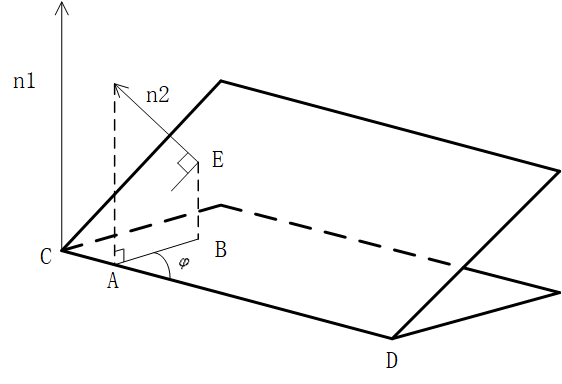
\includegraphics[scale=0.9]{21}
	\caption{证明图}
\end{figure}

由图(19)可以得到直线$CD$是坡面与水平面的交线, $n_1$为水平面的法向量,$n_2$为坡面的法向量,直线 $AB$是坡面法线$n_2$在水平面上的投影与直线$CD$相交于点$A$。因为$n_2$是坡面的法向量,可以推出$n_2$垂直玉坡面,又因为$CD$属于坡面,所以$n_2$垂直于$CD$。同理可得直线$CD$垂直与$n_1$,显然,对法向量$n_1$进行平移,与直线$AB$和法向量$n2$共同构成平面$ABE$。依据直线与平面垂直判定定理:一条直线与一个平面内的两条相交直线都垂直,则该直线与此平面垂直,可以得到直线$CD$垂直于平面$ABE$。又因为直线$AB$属于平面$ABE$,所以我们得出结论,直线$AB$垂直于直线$CD$。据此,我们建立了如图(8)所示的坐标系。











\end{document}